%!TEX root = main.tex

\section{Data}\label{sec:data}

%low-resolution ($\lambda/\Delta\lambda \sim 40$) spectra for $\sim 300,000$ objects
%targeted $80\%$ of galaxies in these fields with $i < 22$
%IMACS instrument \citep{Bigelow03} on Magellan-I Baade 6.5 m telescope to observe $\sim 2,500$ objects at once using a slitmask that covered 0.18 $\degsq$
%statistically-complete sample of $\sim120,000$ spectroscopic redshifts to $i_{\mathrm{AB}}\sim23.5$
%redshifts are derived by fitting a large suite of galaxy, broad-line AGN, and stellar spectral templates to the low-resolution spectra and optical photometry \citep[see][for details]{Cool13}
%objects are classified as galaxies, broad-line AGN or stars depending on the best $\chi^2$ template fit
%redshift precision is ($\sigma_z/(1+z) \sim 0.5\%$)
%low catastrophic outlier rate: less than $3\%$ ($\Delta{z}/(1+z) \ge 0.03$)
%further details of the survey design, targeting, and data see \citet{Coil11}
%further details of the data reduction, redshift confidence, and completeness see \citet{Cool13}

\subsection{PRIMUS}\label{sec:PRIMUS}
 
The PRIsm MUlti-Object Survey (PRIMUS) is the largest faint galaxy intermediate-redshift survey completed to date.
The survey was conducted with the IMACS spectrograph (Bigelow \& Dressler 2003) on the Magellan I Baade 6.5-meter telescope at Las Campanas Observatory with a slitmask and low-dispersion prism.
The design allowed for $\sim~2000$ objects per slitmask to be observed simultaneously with a spectral resolution of ${\lambda/\Delta\lambda \sim 40}$.
Usually two slitmasks were used for each pointing.
PRIMUS obtained robust redshifts $({Q \ge 3}$, see Coil et al.~(2011)) for $\sim120,000$ objects at ${z \sim 0\textendash1.2}$ with a redshift precision of ${\sigma_{z}/(1 + z) \sim 0.005}$.
Objects were targeted to a maximum depth of ${i \ge 23}$.

The total survey area of PRIMUS is $9.1~\degsq$ and encompasses seven distinct science fields: the Chandra Deep Field South-SWIRE field (CDFS), the 02hr and 23hr DEEP2 fields, the COSMOS field (Scoville et al.~2007), the European Large Area ISO Survey-South 1 field (ES1; Oliver et al.~2000), the Deep Lens Survey (DLS; Wittman et al.~2002) F5 field, and two spatially adjacent subfields of the XMM-Large Scale Structure Survey field (XMM-LSS; Pierre et al.~2004). The XMM subfields are the Subaru/XMM-Newton DEEP Survey field (XMM-SXDS; Furusawa et al.~2008) and the Canada-France-Hawaii Telescope Legacy Survey (CFHTLS) field (XMM-CFHTLS).
They were treated separately in our analysis because they were targeted by PRIMUS using different photometric catalogs.
PRIMUS also includes an additional four calibration fields with prior, high resolution spectroscopic redshifts.
Full details of the survey design, targeting, and data summary can be found in Coil et al.~(2011), white details the of data reduction, redshift fitting, precision, and survey completeness are available in Cool et al.~(2013).

Our sample for this study is contained within the PRIMUS fields that also have deep multi-wavelength ultraviolet (UV) imaging from the Galaxy Evolution Explorer (GALEX; Martin et al.~2005), mid-infrared imaging from the Spitzer Space Telescope (Werner at al.~2004) Infrared Array Camera (IRAC; Fazio et al.~2004), and optical and near-IR imaging from various ground-based surveys.
This includes the CDFS, COSMOS, ES1, XMM-CFHTLS, and XMM-SXDS fields, totaling ${\sim 5.5~\degsq}$ of the sky.

\begin{figure*}
  \centering
%  \epsscale{1.0}
%  \epstrim{0.0in 0.5in 0.2in 0.6in}
%  \fbox{\plotone{figures/cone_diagrams}}
%  \plotone{figures/cone_diagrams.eps}
%  \fbox{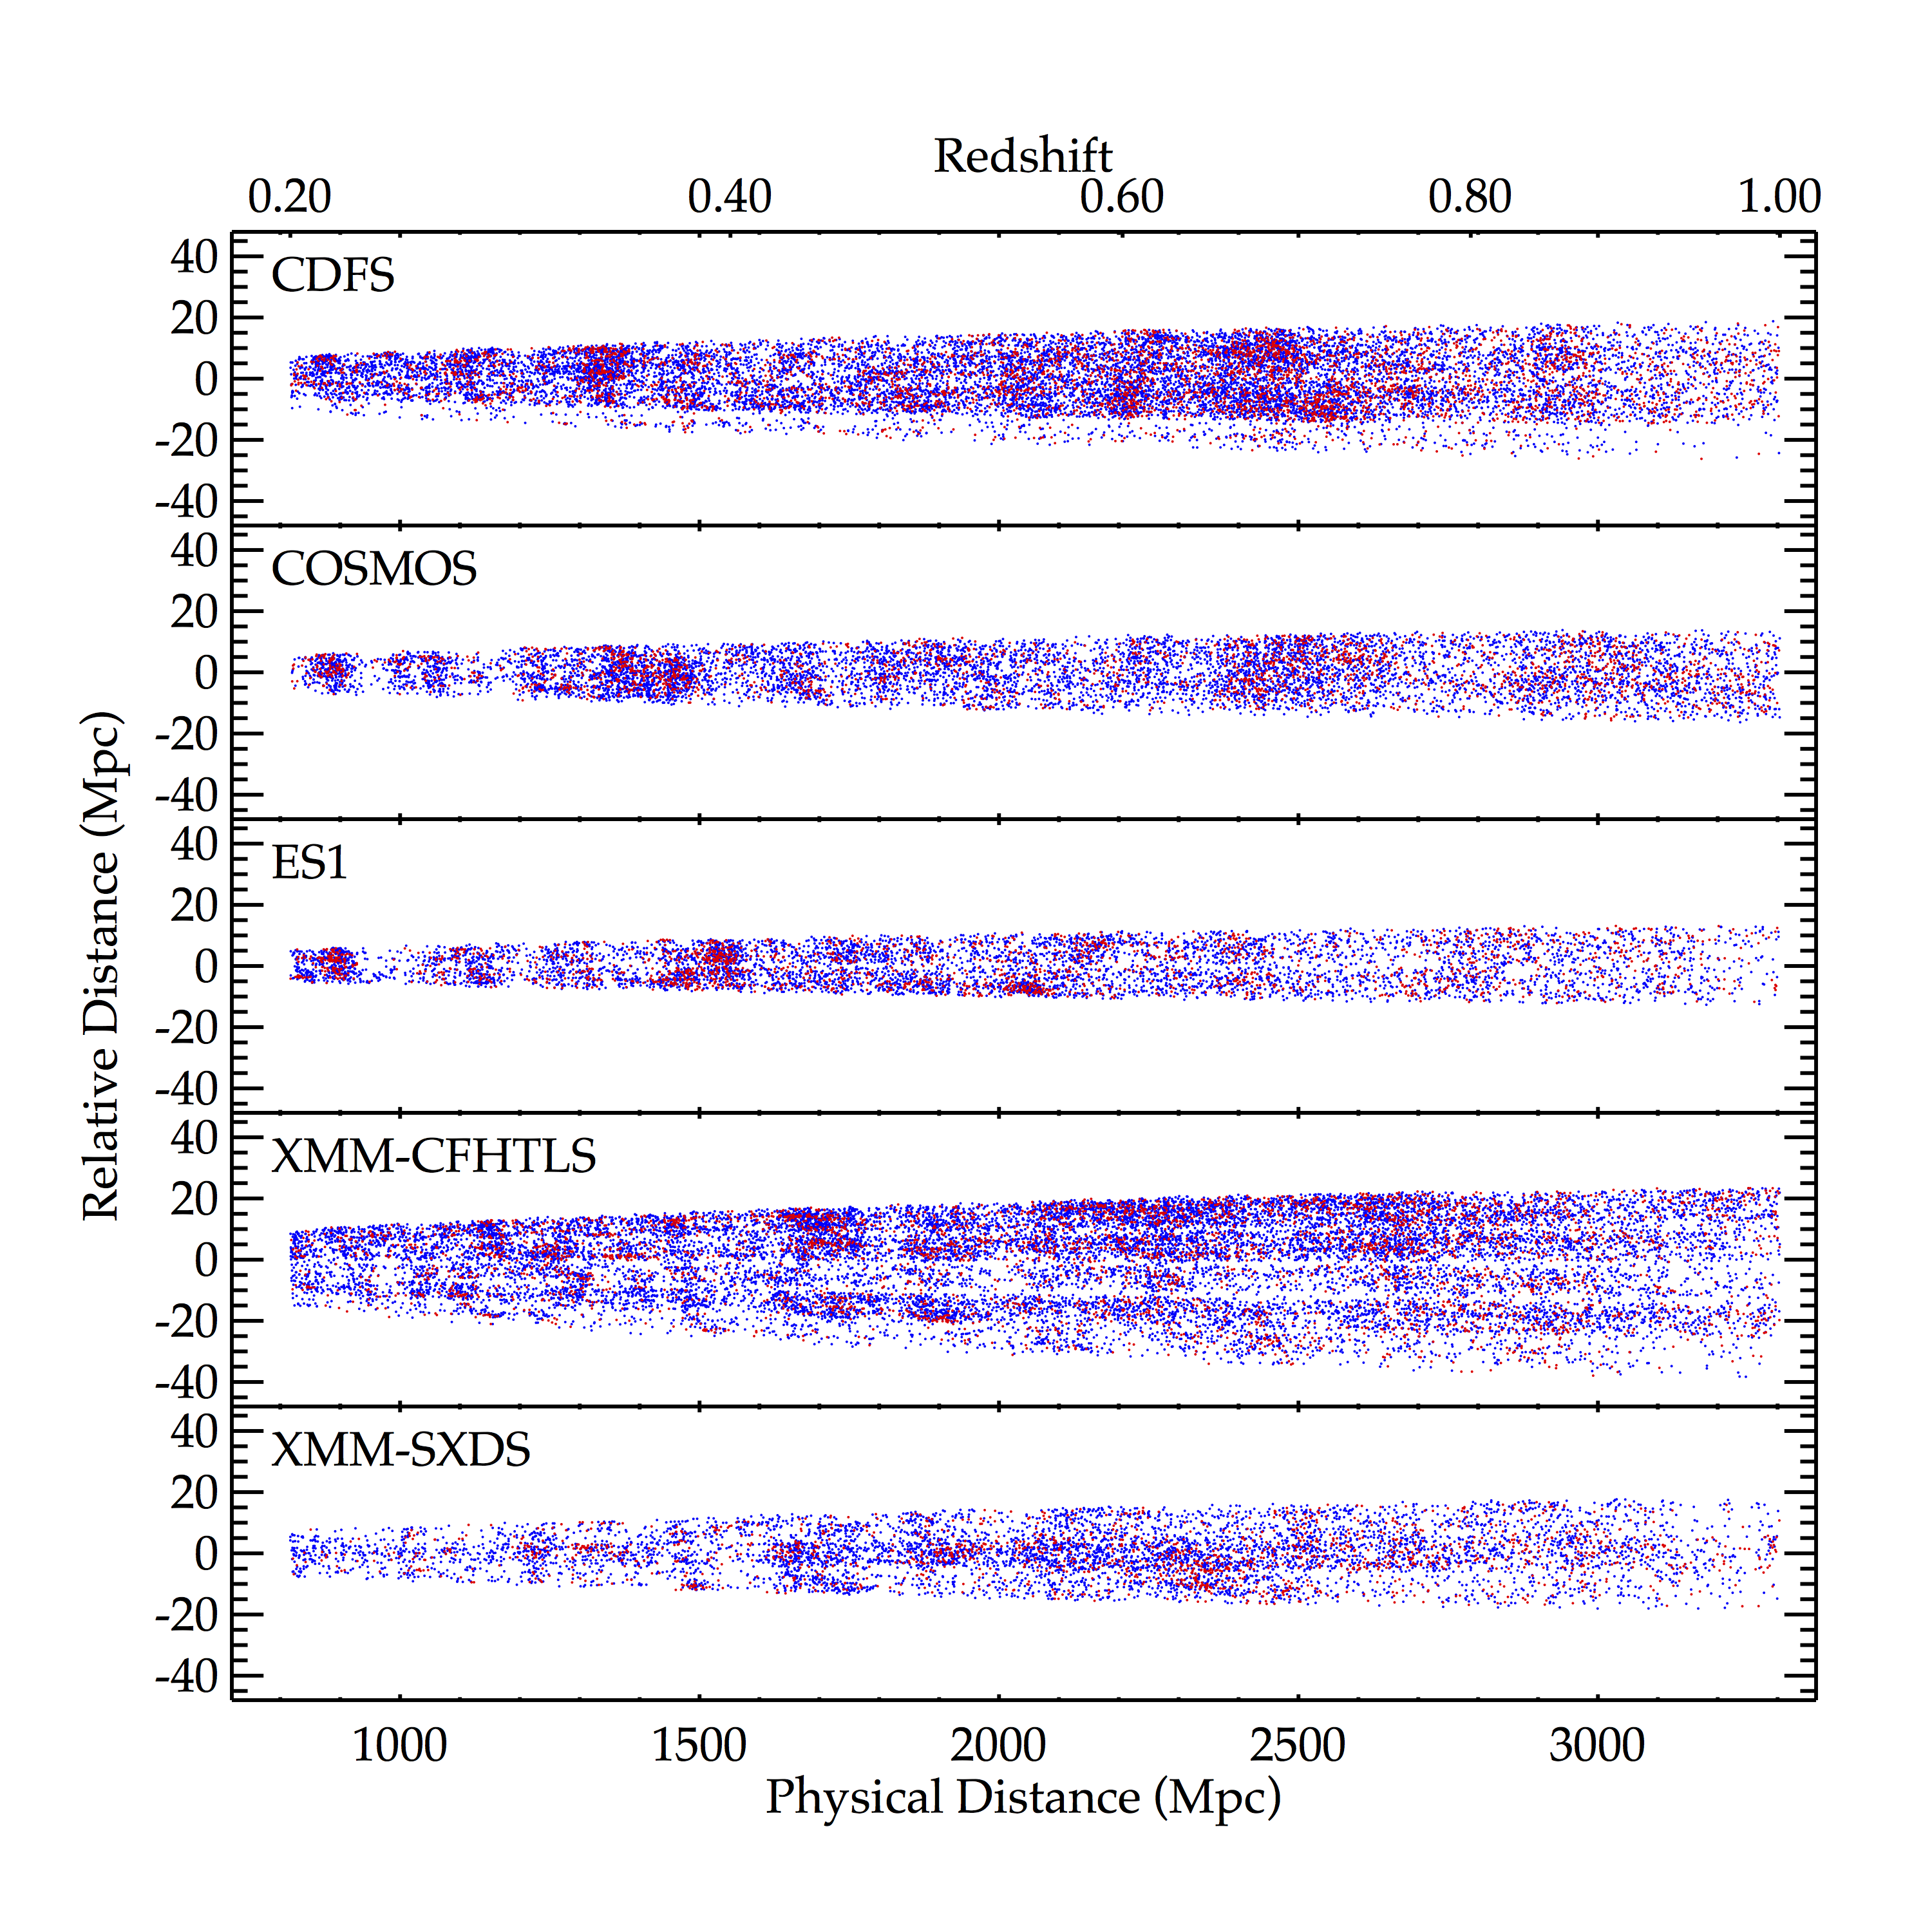
\includegraphics[width=0.9\textwidth,natwidth=600,trim={0.2in 0.5in 0.4in 0.6in},clip]{figures/cone_diagrams.png}}
  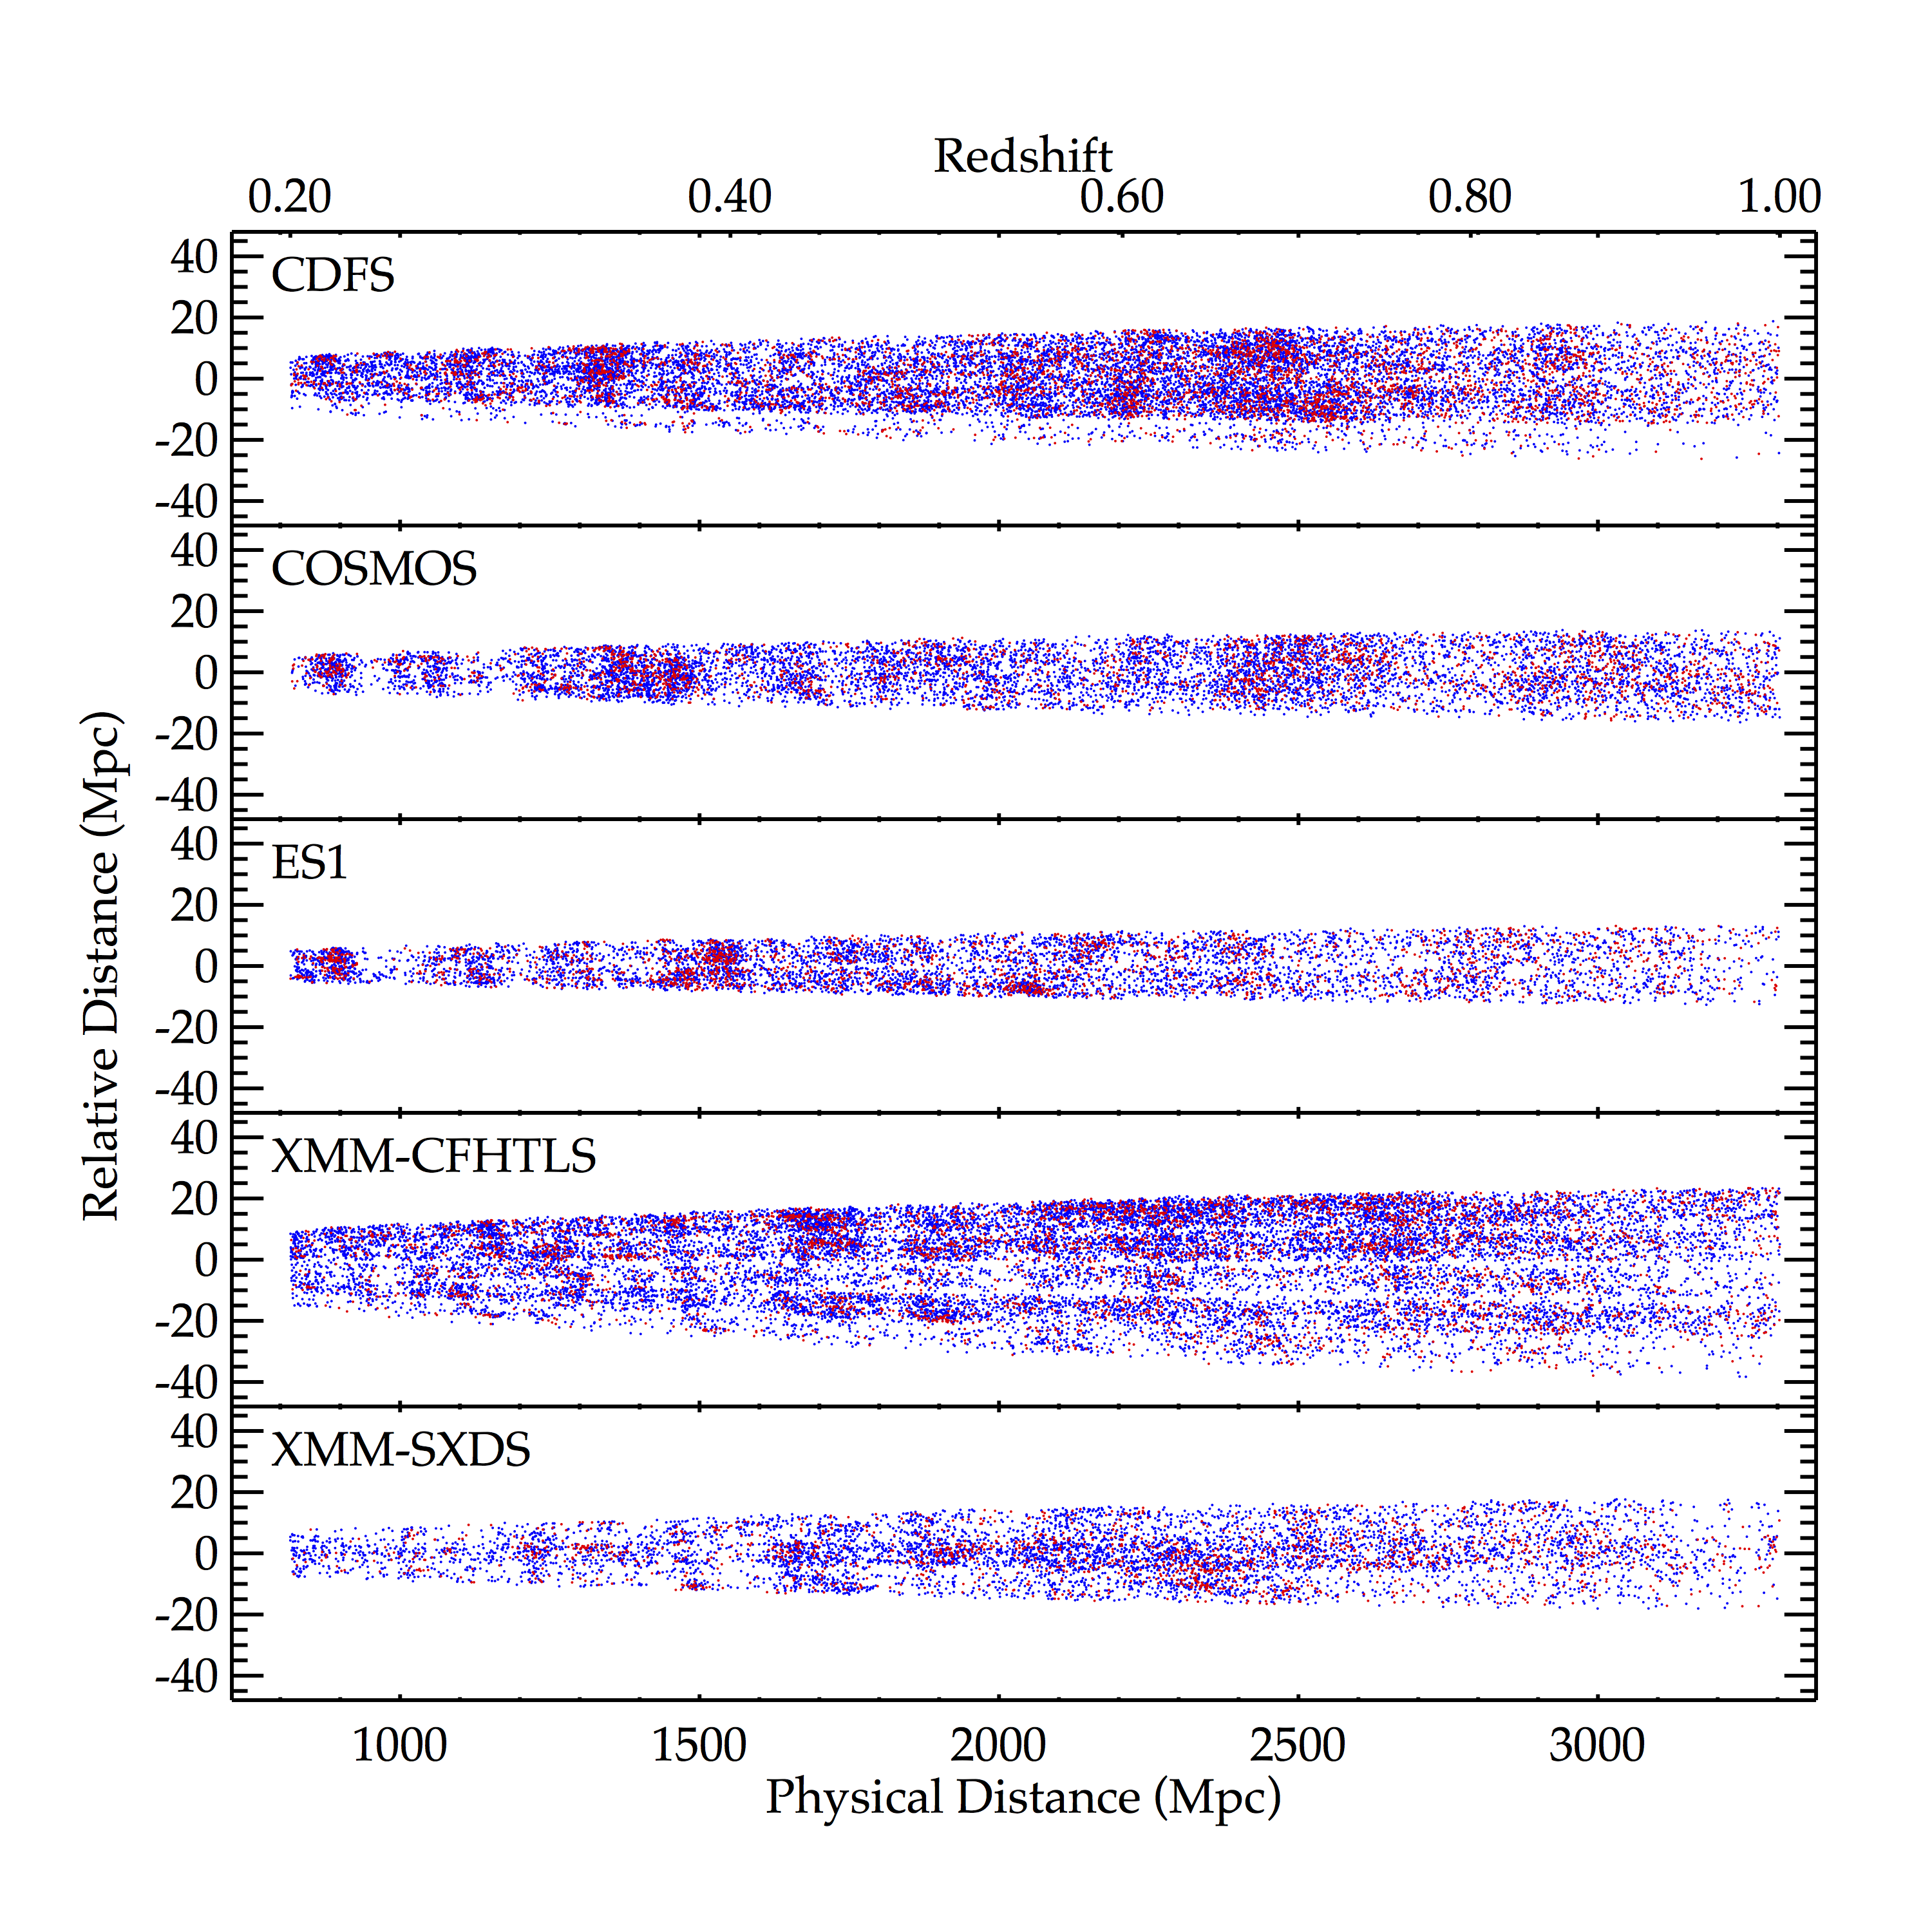
\includegraphics[width=0.9\textwidth,natwidth=600,trim={0.2in 0.5in 0.4in 0.6in},clip]{figures/cone_diagrams.png}
  \caption{Redshift-space distributions of galaxies as a function of physical distance along the line-of-sight and right ascension, relative to the median RA of the field.
From top to bottom the corresponding fields are CDFS, COSMOS, ES1, XMM-CFHTLS, and XMM-SXDS.
Only galaxies with robust redshifts ${(Q \ge 3)}$ are shown.
Star-forming galaxies are shown in blue and quiescent galaxies in red (see~\S\ref{sec:SFQ} and Figure~\ref{fig:SFR_vs_mass}).
}
  \label{fig:cone_diagrams}
\end{figure*}

\subsection{Targeting Weights and Completeness}\label{sec:targ_weight}
 
Within our five selected fields, our sample consists of the ${\sim 60,000}$ galaxies with robust redshifts in the \emph{primary} PRIMUS sample.
The primary sample is composed of galaxies with a well-understood spatial selection function from which a statistically complete sample can be created.
Galaxies are sufficiently clustered in the densest PRIMUS survey regions that two slitmasks per pointing would still under-sample those regions.
Each PRIMUS target was therefore given a density-dependent selection weight that accounts for how many other objects would collide with the target.
Slitmasks were designed to avoid slit collisions by selecting a subsample of targets whose slits don't overlap, while incompleteness in the observations can be corrected by considering the targeting weight of each object.

\subsection{Stellar Mass and SFR Measurements}\label{sec:SFR}
 
Objects in PRIMUS are classified as galaxies, stars, or broad-line active galactic nuclei by fitting low-resolution spectra and multi-wavelength photometry of the objects with an empirical library of templates.
Stellar masses and star formation rates (SFRs) for galaxies with the necessary photometric coverage were measured using \iSEDfit, a suite of routines that uses galaxy redshifts and photometry to compute the statistical likelihood of a large ensemble of model spectral energy distributions (SEDs).
The full details of \iSEDfit are available in Moustakas et al.~(2013).

%\section{Methods}\label{sec:methods}

\subsection{Identifying Star-Forming and Quiescent Galaxies}\label{sec:SFQ}

Our sample is divided into star-forming and quiescent galaxies based on each galaxy's position relative to the star formation (SF) sequence (Noeske et al.~2007), the correlation between SFR and stellar mass exhibited by star-forming galaxies to at least ${z \sim 2}$ (Oliver et al.~2010; Karim et al.~2011 (sources from Moustakas et al.~2013)).
Figure~\ref{fig:SFR_vs_mass} plots SFR vs.~stellar mass in six redshift bins from ${z=0.2\textendash1}$.
The dashed line (Eq.~\ref{eq:SFR}) in each bin bisects the minimum of the bimodal galaxy distribution in that bin, and is given by the following linear relation:

\begin{equation}\label{eq:SFR}
\log\,({\rm SFR}) = -1.29 + 0.65\,\log\,(\mass - 10) + 1.33\,(z - 0.1)
\end{equation}

\noindent where SFR is in units of $\sfrunit$ and $\mass$ is in $\msun$ \todo{needs justification}.
Each galaxy is classified as star-forming or quiescent based on whether its SFR and stellar mass place it above or below the SFR defined by Equation~\ref{eq:SFR}, evaluated at the redshift of the galaxy.

\begin{figure}
  \centering
%  \fbox{\includegraphics[width=\linewidth,natwidth=600,trim={0.1in 0.1in 0.2in 0.6in},clip]{figures/SFR_vs_mass}}
  \includegraphics[width=\linewidth,natwidth=600,trim={0.1in 0.1in 0.2in 0.6in},clip]{figures/SFR_vs_mass}
%  \epsscale{1.1}
%  \epstrim{0.1in 0.1in 0.2in 0.6in}
%  \fbox{\plotone{figures/SFR_vs_mass}}
%  \plotone{figures/SFR_vs_mass}
  \caption{\todo{mention equation of dashed line} Specific star formation rate vs.~stellar mass in six redshift bins from ${z=0.2\textendash1}$.
We divide our sample into star-forming or quiescent according to whether they lie above or below the dashed line, respectively.
This line is parallel to the star formation sequence and evolves with redshift according to Equation~\ref{eq:SFR}.
}
  \label{fig:SFR_vs_mass}
\end{figure}

\subsection{Isolated Primary Sample}\label{sec:IPsample}

Any galaxy in our full sample was considered an isolated primary (IP) candidate if there are no other galaxies 
(i) within a projected distance of 500~kpc from the IP candidate,
(ii) within ${\pm 2.0\,\sigma_{z}\,(1 + z_{\rm IP})}$ in redshift space from the IP candidate \todo{needs justification: 2.0 chosen to maximize S/N by including as many true neighbors as possible while simultaneously minimizing interlopers; also integrate over peculiar velocities}, and
(iii) with stellar mass greater than half the stellar mass of the IP candidate (following Kauffmann et al.~(2013)).
Additionally, IPs can be neighbors of other IPs, and all galaxies can be a neighbor of any number of IPs.

It is possible for galaxies near an edge of the survey area to be falsely classified as isolated if they have any sufficiently massive neighbor(s) within 500~kpc (projected) but just outside the survey area.
To test for this effect We visually inspected the distribution of IPs near survey edges and concluded that false detections near edges do not significantly impact our IP sample.

\subsubsection{Stellar Mass Completeness Limits}\label{sec:mass_compare}

Because PRIMUS is a flux-limited survey, galaxies with high SFRs (i.e.~bluer galaxies) can be detected at higher redshifts than low SFR (redder) galaxies of the same stellar mass.
This introduces a bias toward star-forming galaxies in the PRIMUS sample.
To account for this bias we define a stellar mass limit above which all galaxies can be detected, regardless of their SFR.
This mass completeness limit is a function of redshift, and also varies slightly among fields.
Details of the calculation of PRIMUS mass completeness limits can be found in Moustakas et al.~(2013).
In addition to the isolation criteria described above, all IP candidates must have stellar masses above the completeness threshold of their redshift and field.
Of the 60,071 galaxies in our full sample, 14,888 star-forming and 6,847 quiescent galaxies meet the isolation and stellar mass completeness criteria to be an IP candidate.

\subsubsection{Matching Stellar Mass and Redshift}\label{sec:IPsample_matching}

While our star-forming and quiescent IP candidate populations are statistically complete, their median stellar masses and median redshifts are different because blue and red galaxies of the same stellar mass are detectable to different redshift limits.
Our star-forming (quiescent) IP candidate population has a median stellar mass of 10.44 (10.86) and median redshift of 0.55 (0.60).

To compare the late-type fraction of neighbors around star-forming and quiescent IP galaxies we require star-forming and quiescent IP samples with the same stellar mass and redshift distribution.
To obtain these ``matched'' IP samples, we applied to our IP candidate sample an upper stellar mass cut derived from the PRIMUS stellar mass function (SMF) $\Phi$ for star-forming galaxies (Moustakas et al.~2013).
Specifically, we eliminated all IP candidates (both star-forming and quiescent) with stellar masses greater than the stellar mass at which ${\log\,(\Phi \,/\, 10^{-4}\,\text{Mpc}^{-3}\,\text{dex}^{-1}) \le -3.7}$, interpolated at the redshift of each galaxy.
These upper mass limits are listed in Table~\ref{table:SMFlimit}.

%!TEX root = ../main.tex
\setlength{\tabcolsep}{0.1in}
\begin{deluxetable}{cc}
\tablewidth{0pc}
\tablecolumns{2}
\tablecaption{Matched IP sample stellar mass upper limits.
%$\log\,(\mlim/\msun)$ is the stellar mass in each redshift range where ${\log\Phi=-3.7}$.
%\tablenotemark{a}
\label{table:SMFlimit}
}
\tablehead{
%\multicolumn{1}{c}{} & \multicolumn{4}{c}{Area [deg$^2$]} & \multicolumn{6}{c}{Sample Size} \\
\colhead{Redshift Range} & \colhead{$\log\,(\mmax / \msun)$} }
\label{table:SMFlimit}
\startdata
$0.20-0.30$ & 11.154 \\
$0.30-0.40$ & 11.208 \\
$0.40-0.50$ & 11.255 \\
$0.50-0.65$ & 11.241 \\
$0.65-0.80$ & 11.308 \\
$0.80-1.00$ & 11.324 \\
%\hline \\[-2ex]
\enddata
%\tablenotetext{a}{$\mlim$ is the stellar mass in each redshift range where ${\log\Phi=-3.7}$.}
\end{deluxetable}


We then divided the redshift range and remaining stellar mass range of the quiescent IP candidate population into a grid.
For each of our five fields, from each grid box we randomly selected with replacement the same number of star-forming IP candidates as there are quiescent IPs in that box.
Selection was done separately in each field to account for variation in the stellar mass and redshift distributions of the IP candidate populations in each field.
Our final matched IP sample contains $6,197$ unique quiescent and $4,185$ unique star-forming IPs.
Each star-forming IP was assigned a weight equal to the number of times it was randomly selected while matching the distribution of the quiescent IP sample.
The sum of all star-forming IP weights equals the total number of unique quiescent IPs.
Figure~\ref{fig:IPsample_matched} plots stellar mass vs.~redshift for all star-forming and quiescent galaxies in our sample, 
as well as the stellar mass vs.~redshift distribution of our final ``matched'' IP sample.
In Figure~\ref{fig:IPhist_latefrac_vs_z} we show the redshift distributions of all star-forming (solid blue line) and quiescent (dashed red line) IPs, and the late-type fraction of all PRIMUS galaxies in our full sample as a function of redshift.

\begin{figure}
  \epsscale{1.1}
  \epstrim{0.4in 0.2in 0.2in 0.4in}
  \fbox{\plotone{figures/matchedSamplePlot_allFields}}
%  \plotone{figures/matchedSamplePlot_allFields}
  \caption{Stellar mass vs.~redshift for all star-forming galaxies in our sample (blue contours), all quiescent galaxies (red contours) in our sample, and the combined subsets of the star-forming and quiescent IP candidate populations with matching stellar mass and redshift distributions (gray shaded contours).
The gray contours show the distribution of our final ``matched'' IP sample.
}
  \label{fig:IPsample_matched}
\end{figure}

\begin{figure}
  \epsscale{1.1}
  \epstrim{0.1in 0.1in 0.5in 0.8in}
%  \fbox{\plotone{figures/IPhist_latefrac_vs_z}}
  \plotone{figures/IPhist_latefrac_vs_z}
  \caption{Top panel: Redshift distributions of all star-forming (blue) and quiescent (red) IPs.
Bottom panel: Late-type fraction of all PRIMUS galaxies in our full sample as a function of redshift.
}
  \label{fig:IPhist_latefrac_vs_z}
\end{figure}

%FIELD	MAX WGT	weight fraction = 1
%cdfs		6	0.658472
%XMM-CFHTLS	7	0.691321
%cosmos		6	0.651163
%es1		7	0.623077
%xmm-sxds	9	0.676667

The importance of matching both the stellar mass and redshift distributions of our IP sample is illustrated in Figure~\ref{fig:IPsample_compare},
which shows how the late-type fractions of neighbors of star-forming and quiescent IPs (see \S\ref{sec:LTfraction}) differ when different IP samples are used.
Figure~\ref{fig:IPsample_compare} plots the fraction of neighbors of star-forming and quiescent IPs that are late-type as a function of projected distance from the IP in 1~Mpc annuli out to 15~Mpc for four different IP samples.
%
In panel (a) all IP candidates above the M13 mass completeness limit (\S\ref{sec:mass_compare}) are included.
Here the median stellar mass of the quiescent IP population is 0.42~dex greater than that of the star-forming IP population, and the median redshift is greater by 0.05.
This difference in stellar mass distribution means that star-forming IPs are preferentially located in a region of Figure~\ref{fig:IPsample_matched} where the PRIMUS sample of early-type galaxies is incomplete, causing us to overestimate the neighbor late-type fraction for star-forming IPs (at all projected distances).
The result is a relatively fixed offset between the solid and dashed lines in Figure~\ref{fig:IPsample_compare}(b) that persists to the largest projected distances we can measure with PRIMUS (we show to 15 Mpc, but can go to roughly double that before edge effects take over), mimicking a conformity signal.
%
In panel (b) we select star-forming and quiescent IP samples with matched redshift distributions using the method described in \S\ref{sec:IPsample_matching}.
This reduces the median stellar mass difference between the IP samples to 0.3~dex, although a smaller fixed offset remains at all projected distances.
%
In panel (c) we select star-forming and quiescent IP samples with matched stellar mass distributions, resulting in a star-forming IP sample with a higher median redshift than that of the quiescent IP sample.
In this case the systematic bias mimics the opposite of a conformity signal; the solid line moves closer to the dashed line at all projected distances, actually dropping below it at $>5$~Mpc.
%
Finally, panel (d) shows results for our matched stellar mass and matched redshift IP sample.
Failure to control for one or both of stellar mass and redshift introduces bias into the relative neighbor late-type fractions of star-forming and quiescent IPs.
Only by matching both the stellar mass and redshift distributions of our star-forming and quiescent IP samples do we eliminate the systematic bias in neighbor late-type fraction measurements that could masquerade as a conformity signal.

\begin{figure*}
  \epsscale{1.0}
  \epstrim{0.1in 0.3in 0.4in 0.8in}
%  \fbox{\plotone{figures/unmatchedIPsampleCompare}}
  \plotone{figures/unmatchedIPsampleCompare}
  \caption{Neighbor late-type fractions to ${\Rproj<15}$~Mpc for star-forming and quiescent IPs for four different IP samples: 
(a)~all IP candidates above the M13 mass completeness limit (\S\ref{sec:mass_compare});
(b)~matched redshift distribution only;
(c)~matched stellar mass distribution only;
(d)~matched stellar mass and redshift distribution.
The median redshift and stellar mass of both IP samples are also shown in each panel.
}
  \label{fig:IPsample_compare}
\end{figure*}
